\documentclass[a4paper,12pt]{article}
\usepackage[english,portuges,brazil]{babel}
\usepackage[utf8]{inputenc} % permite caracteres
\usepackage[T1]{fontenc}	% permite melhor hifenização para Português/Espanhol
% \usepackage{ae}     % Melhora padrão do tamanho das fontes e zoom (exige babel)
%\usepackage[round,authoryear]{natbib}	% Utilizado para bibliografia
%\usepackage{ucs}	% Inclui utf-8 (caso utilize latin1 no inputec)
%\usepackage[round,authoryear]{natbib}	% Pacote completo para bibliografia (não usaremos)
%\usepackage{cite}	% Pacote para citação, não precisa!

\usepackage{fancyhdr}
\usepackage{fullpage}
\usepackage{indentfirst}    % Identa também o primeiro parágrafo das seções!
\usepackage{caption}
\usepackage{tikz}
\usetikzlibrary{shapes,arrows}
\usepackage[RPvoltages]{circuitikz}
\usepackage{url}
\usepackage{graphicx}
\usepackage{subcaption}
\usepackage[table]{xcolor}
\usepackage{booktabs}

% Para tabelas longas
\usepackage{booktabs}
\usepackage{longtable}
\usepackage{array}
\usepackage{ragged2e}

\newcolumntype{L}[1]{>{\RaggedRight\arraybackslash}p{#1}}

\usepackage{amsmath}	%permite equações matemáticas
\usepackage{amsfonts}   %fontes especiais para matemática
\usepackage{amssymb}    %símbolos especiais para matemática

\usepackage{graphicx}	%permite inclusão de figuras
%\usepackage{graphpap}   %papel gráfico
\usepackage[final]{pdfpages}  % Permite incluir PDF pronto no documento

% Define título
\newcommand{\printprof}{Prof. Dr. Eduardo Noronha de Andrade Freitas}
\newcommand{\printtitle}{Otimização de dietas de custo mínimo para bovinos leiteiros com o simulador RuFaS e programação linear}
\newcommand{\printsubject}{Modelagem e Otimização Aplicada}
\newcommand{\printauthor}{Afrain da Silva Calixto\\Flávio Lourenço da Silva\\Gustavo Adolpho Souteras Barbosa}
\newcommand{\printkeywords}{programação linear,Simplex,RuFaS,nutrição animal,IFG}


% Define algumas cores
\usepackage{color}
\definecolor{dkgreen}{rgb}{0,0.6,0}
\definecolor{gray}{rgb}{0.9,0.9,0.9}
\definecolor{mauve}{rgb}{0.58,0,0.82}
\definecolor{mylinkcolor}{rgb}{0,0,0}

%permite hyperlink e alterar suas configurações
\usepackage[pdftex,
  pdftitle={\printtitle},
  pdfsubject={\printtitle},
  pdfauthor={\printauthor},
  pdfkeywords={trabalho, exemplo, modelo},
  pdfcreator={Modelo do \printprof},
  pdfproducer={LaTeX},
  pdflang=pt-BR,
  pdfborder={0 0 0},
  colorlinks=true, urlcolor=mylinkcolor, citecolor=mylinkcolor,
  anchorcolor=mylinkcolor, linkcolor=mylinkcolor]{hyperref}

%\usepackage{francyvrb} % Verbagin
% ============================================================
% Listings - configuração para códigos-fonte
% ============================================================
\usepackage[utf8]{inputenc}
\usepackage{xcolor}
\usepackage{listings}
\usepackage{scrbase}
\usepackage{float}

% Nome da listagem em português
\newcaptionname{portuguese}{\lstlistingname}{Código}

% ------------------------------------------------------------
% Configuração de caracteres especiais
% ------------------------------------------------------------
\lstset{
    inputencoding=utf8,
    extendedchars=true,
    literate=
        {ä}{{\"a}}1
        {Ä}{{\"A}}1
        {á}{{\'a}}1
        {Á}{{\'A}}1
        {à}{{\`a}}1
        {À}{{\`A}}1
        {ã}{{\~a}}1
        {Ã}{{\~A}}1
        {â}{{\^a}}1
        {Â}{{\^A}}1
        {ë}{{\"e}}1
        {Ë}{{\"E}}1
        {é}{{\'e}}1
        {É}{{\'E}}1
        {è}{{\`e}}1
        {È}{{\`E}}1
        {ê}{{\^e}}1
        {í}{{\'i}}1
        {Í}{{\'I}}1
        {ì}{{\`i}}1
        {Ì}{{\`I}}1
        {ç}{{\c{c}}}1
        {Ç}{{\c{C}}}1
        {ğ}{{\u{g}}}1
        {Ğ}{{\u{G}}}1
        {ö}{{\"o}}1
        {Ö}{{\"O}}1
        {ó}{{\'o}}1
        {Ó}{{\'O}}1
        {ò}{{\`o}}1
        {Ò}{{\`O}}1
        {õ}{{\~o}}1
        {Õ}{{\~O}}1
        {ô}{{\^o}}1
        {Ô}{{\^O}}1
        {ş}{{\c{s}}}1
        {Ş}{{\c{S}}}1
        {ü}{{\"u}}1
        {Ü}{{\"U}}1
        {ú}{{\'u}}1
        {Ú}{{\'U}}1
        {ù}{{\`u}}1
        {Ù}{{\`U}}1
        {Ú}{{\'U}}1
        {→}{{$\rightarrow$}}1
        {━}{{-}}1
}

% ------------------------------------------------------------
% Cores
% ------------------------------------------------------------
\definecolor{codebg}{rgb}{0.94,0.94,0.94}
\definecolor{codeborder}{rgb}{0.70,0.70,0.70}
\definecolor{codegreen}{rgb}{0.00,0.50,0.00}
\definecolor{codeblue}{rgb}{0.00,0.20,0.70}
\definecolor{codegray}{rgb}{0.40,0.40,0.40}
\definecolor{codemauve}{rgb}{0.58,0.00,0.82}

% ------------------------------------------------------------
% Configuração geral
% ------------------------------------------------------------
\lstset{
    basicstyle=\footnotesize\ttfamily,
    showstringspaces=false,
    breaklines=true,
    keepspaces=true,
    tabsize=4,
    numbers=left,
    numberstyle=\tiny\color{codegray},
    numbersep=5pt,
    frame=single,
    rulecolor=\color{codeborder},
    backgroundcolor=\color{codebg},
    xleftmargin=6pt,
    xrightmargin=6pt
}

% ============================================================
% Assembly
% ============================================================
\lstdefinelanguage[x8051]{Assembler}
[x86masm]{Assembler}
{
    morekeywords={
        clr, movc, movx, ljmp, sjmp, lcall,
        cjne, djnz, swap, orl, subb, rl,
        anl, xch
    },
    sensitive=false,
    deletekeywords={loop,low,dl}
}

\lstdefinestyle{assembly}{
    language=[x8051]Assembler,
    basicstyle=\footnotesize\ttfamily,
    keywordstyle=\color{codeblue},
    commentstyle=\color{codegreen},
    stringstyle=\color{codemauve},
    backgroundcolor=\color{codebg},
    frame=single,
    rulecolor=\color{codeborder},
    breaklines=true,
    showstringspaces=false,
    tabsize=4,
    numbers=left,
    numberstyle=\tiny\color{codegray},
    numbersep=5pt
}

% ============================================================
% Python
% ============================================================
\lstdefinestyle{python}{
    language=Python,
    basicstyle=\scriptsize,
    keywordstyle=\color{codeblue},
    stringstyle=\color{codemauve},
    commentstyle=\color{codegreen}\itshape,
    backgroundcolor=\color{codebg},
    frame=single,
    rulecolor=\color{codeborder},
    breaklines=true,
    showstringspaces=false,
    keepspaces=true,
    tabsize=4,
    numbers=left,
    numberstyle=\tiny\color{codegray},
    numbersep=5pt,
    xleftmargin=6pt,
    xrightmargin=6pt
}

% ============================================================
% MicroPython
% ============================================================
\lstdefinestyle{micropython}{
    language=Python,
    basicstyle=\footnotesize\ttfamily,
    keywordstyle=\color{codegreen},
    stringstyle=\color{codeblue},
    commentstyle=\color{codegray}\itshape,
    backgroundcolor=\color{codebg},
    frame=single,
    rulecolor=\color{codeborder},
    framerule=0.5pt,
    breaklines=true,
    showstringspaces=false,
    keepspaces=true,
    tabsize=4,
    numbers=left,
    numberstyle=\tiny\color{codegray},
    numbersep=5pt,
    xleftmargin=6pt,
    xrightmargin=6pt
}

% ============================================================
% SQL
% ============================================================
\lstdefinestyle{sql}{
    language=SQL,
    basicstyle=\scriptsize,
    keywordstyle=\color{codeblue},
    stringstyle=\color{codemauve},
    commentstyle=\color{codegreen}\itshape,
    backgroundcolor=\color{codebg},
    frame=single,
    rulecolor=\color{codeborder},
    breaklines=true,
    showstringspaces=false,
    keepspaces=true,
    tabsize=4,
    numbers=left,
    numberstyle=\tiny\color{codegray},
    numbersep=5pt,
    xleftmargin=6pt,
    xrightmargin=6pt
}

% Margens superiores e esquerda
\hoffset        = -1.74cm   % Offset da margem esquerda
\oddsidemargin  = +0.00cm   % Separação da margem esquerda com meio
\marginparsep   = +0.00cm   % Separação da margem esquerda com fim
\marginparwidth = +0.00cm   % Simetria da margem esquerda
\marginparpush  = +0.00cm   % Simetria da margem esquerda
\voffset        = -1.54cm   % Offset da margem superior
\topmargin      = +0.00cm   % Espaço superior após a margem

% Cabeçalho e rodapé
\footskip   = 1.25cm    % Espaço da margem inferior, incluindo rodapé
\headheight = 3.00cm    % Cabeçalho
\headsep    = 0.50cm    % Separação entre cabeçalho e texto

% Área do texto útil
\textheight = 23.15cm   % Altura do texto
\textwidth  = 19.40cm   % Largura do texto
\headwidth  = 19.40cm   % Largura do cabeçalho

\usepackage{lastpage}
\pagestyle{fancy}
%\lhead{\includegraphics[height=2.5cm]{ifg-imagem-resumida}}
\lhead{
\includegraphics[height=2.5cm]{ifg-resumida}}
\rhead{
\textbf{
    MINISTÉRIO DA EDUCAÇÃO}\\
    INSTITUTO FEDERAL DE GOIÁS\\
    \printtitle
}
\fancypagestyle{primeira}{
  \renewcommand{\headrulewidth}{0.0pt}
  \renewcommand{\footrulewidth}{0.0pt}
  \footskip   = 0.45cm    % Espaço da margem inferior, incluindo rodapé
  % \fancyhead{}
  % \fancyfoot{}
  \lhead{}
  \chead{}
  \rhead{}
  \lfoot{}
  \cfoot{}
  \rfoot{}
}
%\rhead{ \textbf{\printprof}}
%\rhead{}
%\lfoot{Esquerda do Rodapé}
\cfoot{\thepage\ de \pageref{LastPage}}
%\rfoot{Direita do Rodapé}
\renewcommand{\headrulewidth}{0.50pt}
\renewcommand{\footrulewidth}{0.5pt}



\title{
\vspace{-2em}

\includegraphics[width=.7\textwidth]{ifg-completa.jpg}

\vspace{1em}
\printtitle
\vspace{2cm}

}

\author{
\printauthor
\vspace{2cm} \\
\printprof \\
\vspace{2cm}
}



\begin{document}

\maketitle
\thispagestyle{primeira}
\newpage

\begin{abstract}
O presente documento descreve os procedimentos adotados para formular, por programação linear, a dieta de custo mínimo das vacas em lactação da fazenda sintética Campo Dourado, situada em Goiás, e para avaliar o efeito dessa dieta com o simulador de fazendas leiteiras RuFaS (\textit{Ruminant Farm Systems}). As exigências nutricionais dos animais foram obtidas do próprio simulador, segundo o padrão NASEM (2021), e os preços dos ingredientes foram levantados no mercado brasileiro. O modelo linear reproduz as restrições do otimizador de ração do RuFaS e foi resolvido para um custo de R\$ 24,31 por vaca por dia. A dieta do programa linear foi então simulada no RuFaS para verificar seus efeitos sobre a produção de leite e a emissão de metano.
\end{abstract}

\newpage

% =====================================================================
\newpage
\section{Introdução e objetivo do problema}\label{sec:introducao}

A alimentação é o principal item de custo da produção de leite. Formular a dieta de um rebanho consiste em escolher quanto de cada ingrediente oferecer aos animais de forma que suas necessidades de energia, proteína, minerais e fibra sejam atendidas. Como cada ingrediente tem um preço e uma composição diferentes, existem muitas combinações possíveis, e a escolha da mais barata que ainda atenda a todas as necessidades é um ótimo problema de otimização.

Conforme apresentado em aula \cite{slides:rufas}, uma vaca com cerca de 150 dias de lactação precisa diariamente de uma quantidade de energia, proteína, cálcio, fósforo e fibra, calculada por padrões científicos de exigência nutricional (NRC e NASEM) a partir do peso do animal, da fase de lactação e da produção de leite. A pergunta do produtor é qual é a dieta mais barata que ainda atende a todas essas exigências. Nutrir demais desperdiça dinheiro, porque os nutrientes que a vaca não aproveita viram custo e, às vezes, poluição; nutrir de menos compromete a saúde e a produção de leite. O ponto ótimo, o menor custo que ainda cobre todas as exigências, é o que um otimizador calcula. Além disso, a vaca faz parte de um rebanho, dentro de uma fazenda com solo, lavouras, dejetos, clima e economia interagindo, e é essa fazenda inteira que o RuFaS modela.

Os requisitos do trabalho são desenvolver um módulo de otimização da dieta integrado ao simulador RuFaS, com avaliação do efeito econômico e análise de sensibilidade. Para a fazenda sintética Campo Dourado, situada em Goiás, deve-se minimizar o custo da nutrição avaliando os alimentos (matéria seca, matéria natural etc.) e respeitando as restrições nutricionais já estabelecidas pelo padrão NASEM/NRC adotado no simulador. Os requisitos incluem apresentar:

\begin{enumerate}
    \item o contexto e os dados reais da fazenda;
    \item os parâmetros de entrada que devem ser alterados para otimizar;
    \item a função objetivo;
    \item as restrições, segundo o padrão NASEM;
    \item um modelo pronto para um \textit{solver};
    \item o método Simplex, passo a passo;
    \item o plano de análise de sensibilidade, variando as simulações após o ótimo.
\end{enumerate}

O RuFaS já possui um otimizador de ração, que minimiza o custo com um método de programação não linear. Neste trabalho o mesmo problema é reescrito como um programa linear (PL) e o resultado é comparado com o do simulador.

A integração com o RuFaS foi feita por meio dos arquivos do simulador, sem alterar o seu código. O módulo de otimização é um \textit{script} Python executado à parte, que lê as exigências nutricionais nos arquivos de saída do RuFaS, usa funções do próprio simulador para calcular os coeficientes de energia e proteína e devolve a dieta de custo mínimo ao arquivo de alimentação (\textit{feed.json}), usado pelo RuFaS na simulação seguinte. O otimizador de ração interno do RuFaS não foi substituído: durante a simulação, ele continua reformulando a ração a partir da dieta informada. O fluxo de trabalho adotado está resumido na \textbf{Figura \ref{fig:fluxo}}.

\begin{figure}[htbp]
\centering
\begin{tikzpicture}[
    caixa/.style={rectangle, draw, rounded corners, align=center, minimum width=3.6cm, minimum height=1.1cm, font=\small},
    seta/.style={->, >=stealth, thick}]
    \node[caixa] (planilha) at (0,0)   {Planilha de\\ingredientes e preços};
    \node[caixa] (rufas1)   at (5,0)   {RuFaS\\(caso base)};
    \node[caixa] (exig)     at (10,0)  {Exigências\\nutricionais};
    \node[caixa] (nasem)    at (0,-2.5){Composição\\(NASEM\_Comp.csv)};
    \node[caixa] (pl)       at (5,-2.5){Programa linear};
    \node[caixa] (dieta)    at (10,-2.5){Dieta de\\custo mínimo};
    \node[caixa] (rufas2)   at (10,-5) {RuFaS\\(dieta do PL)};
    \node[caixa] (aval)     at (5,-5)  {Avaliação econômica\\e sensibilidade};
    \draw[seta] (planilha) -- (rufas1);
    \draw[seta] (rufas1) -- (exig);
    \draw[seta] (exig) -- (pl);
    \draw[seta] (planilha) -- (pl);
    \draw[seta] (nasem) -- (pl);
    \draw[seta] (pl) -- (dieta);
    \draw[seta] (dieta) -- (rufas2);
    \draw[seta] (rufas2) -- (aval);
\end{tikzpicture}
\caption{Fluxo de trabalho: o RuFaS fornece as exigências, o programa linear escolhe a dieta e o RuFaS simula o efeito dessa dieta.}
\label{fig:fluxo}
\end{figure}

% =====================================================================
\newpage
\section{O simulador RuFaS}\label{sec:rufas}

O RuFaS é um ambiente de modelagem de código aberto que simula, dia a dia, uma fazenda leiteira inteira: rebanho, alimentação, lavouras, solo, esterco e emissões \cite{website:rufas, website:rufasdocs}. Foi usada a versão 1.0.5 (\textit{commit} \texttt{beac7f321}, de 16 de outubro de 2026). Cada simulação lê um conjunto de arquivos JSON e CSV de entrada, listados num arquivo de metadados, e grava os resultados num CSV com uma coluna por variável.

Uma única chamada de \textit{main.py} dispara a simulação, e o programa lê uma cadeia de arquivos JSON \cite{slides:rufas}. Na fazenda deste trabalho, a cadeia é:

\begin{enumerate}
    \item \textit{\_pipeline\_\allowbreak task\_\allowbreak manager\_\allowbreak metadata.json}: indica o arquivo de tarefas a executar;
    \item \textit{\_pipeline\_tasks.json}: define a tarefa de simulação (tipo, semente aleatória, prefixo dos arquivos de saída);
    \item \textit{farm\_metadata.json}: o arquivo-mestre, que liga os dados do animal, da dieta, da configuração, do clima, das lavouras e do esterco;
    \item \textit{inputs\_resolvidos/}: os arquivos de dados que o usuário edita, como \textit{animal.json}, \textit{feed.json}, \textit{config.json} e \textit{NASEM\_Comp.csv}.
\end{enumerate}

\subsection{Alimentos e rações}

No RuFaS, \textbf{alimento} (\textit{feed}) é cada ingrediente isolado, como silagem de milho ou milho grão, identificado por um número (\textit{rufas\_id}). \textbf{Ração} (\textit{ration}) é a receita, isto é, a mistura de alimentos, em porcentagem da matéria seca, que um grupo de animais consome. O rebanho é dividido em quatro grupos, cada um com sua ração: bezerras (\textit{calf}), novilhas (\textit{growing}), vacas próximas ao parto (\textit{close\_up}) e vacas em lactação (\textit{lac\_cow}).

Os ingredientes se dividem em dois grupos \cite{slides:rufas}: \textbf{volumosos}, fibrosos e com pouca energia, como capins, fenos e silagens, que fornecem fibra e saciedade; e \textbf{concentrados}, com pouca fibra e muita energia ou proteína, como milho moído e farelo de soja. Cada ingrediente tem composição nutricional conhecida e um preço por quilograma, e no RuFaS os valores exatos vêm da biblioteca NASEM ou NRC.

As informações sobre alimentos e rações estão distribuídas em dois arquivos, descritos na \textbf{Tabela \ref{tab:arquivos-dieta}}. Todas as quantidades são expressas em \textbf{matéria seca} (MS), ou seja, o alimento descontado da água. A silagem de milho, por exemplo, tem cerca de 65\% de água; a comparação em matéria seca coloca todos os alimentos na mesma base nutricional.

\begin{table}[htbp]
    \centering
    \caption{Arquivos de entrada relacionados à dieta}
    \label{tab:arquivos-dieta}
    \begin{tabular}{L{4cm}L{12cm}}
        \toprule
        \textbf{Arquivo} & \textbf{Conteúdo} \\
        \midrule
        \rowcolor{gray!15}
        \textit{NASEM\_Comp.csv} & Composição de 176 alimentos segundo o padrão NASEM (2021) \cite{nasem2021}: matéria seca, proteína bruta, fibra (FDN), extrato etéreo, energia, minerais, aminoácidos e limites de inclusão. \\
        \textit{feed.json} & Alimentos disponíveis na fazenda, com o custo de compra (\textit{purchased\_feed\_cost}, por kg de MS), e as rações de cada grupo, em porcentagem da MS. \\
        \bottomrule
    \end{tabular}
\end{table}

\subsection{Formulação da ração no simulador}

As necessidades dos animais (\textbf{exigências}) não são dados de entrada: o RuFaS as calcula durante a simulação, a partir do peso vivo, peso adulto, dia de gestação, escore de condição corporal, dias em lactação, número de partos, produção e composição do leite, entre outros. Essas exigências seguem o padrão nutricional escolhido no arquivo de configuração, que neste trabalho é o NASEM (2021) \cite{nasem2021}; o simulador também oferece o NRC (2001) \cite{nrc2001}.

A cada intervalo de formulação (45 dias nesta fazenda), o RuFaS recalcula as exigências médias de cada grupo e formula a ração. O otimizador interno minimiza o custo da ração com o método SLSQP (\textit{Sequential Least Squares Programming}) da biblioteca SciPy, sujeito às restrições nutricionais \cite{slides:rufas}. Esse otimizador é a classe \textit{RationOptimizer}, e a função objetivo que ele minimiza é a soma, para todos os alimentos, da quantidade multiplicada pelo preço (\textbf{Listagem \ref{lst:objetivo-rufas}}).

\begin{lstlisting}[caption={Função objetivo do otimizador de ração do RuFaS (\textit{ration\_optimizer.py}).}, label={lst:objetivo-rufas}]
def objective(decision_vector, ration_config):
    return float(sum(np.multiply(decision_vector, ration_config.price_list)))
\end{lstlisting}

O comportamento depende do campo \textit{ration.user\_input} do arquivo \textit{animal.json}:

\begin{itemize}
    \item \textbf{\textit{true}}: o otimizador parte da ração informada no \textit{feed.json} e só pode variar cada porcentagem em até $\pm$10\% (\textit{user\_defined\_ration\_tolerance} = 0,1);
    \item \textbf{\textit{false}}: o otimizador escolhe livremente a quantidade de cada alimento disponível para o grupo.
\end{itemize}

Quando nenhuma ração atende às exigências, o simulador reduz a produção de leite esperada das vacas em lactação e tenta novamente.

% =====================================================================
\section{A fazenda Campo Dourado}\label{sec:fazenda}

A fazenda Campo Dourado é uma fazenda sintética, situada em Goiás para fins de simulação, gerada para o RuFaS e fornecida para o trabalho com todos os arquivos de entrada já preenchidos. Seus principais parâmetros estão na \textbf{Tabela \ref{tab:fazenda}}.

\begin{table}[htbp]
    \centering
    \caption{Parâmetros da fazenda Campo Dourado}
    \label{tab:fazenda}
    \begin{tabular}{ll}
        \toprule
        \textbf{Parâmetro} & \textbf{Valor} \\
        \midrule
        \rowcolor{gray!15}
        Cenário & conservador (manejo base) \\
        Rebanho & 100 vacas, das quais 83,56\% em lactação \\
        \rowcolor{gray!15}
        Ordenhas por dia & 3 \\
        Clima & Goiás (arquivo \textit{weather.csv}) \\
        \rowcolor{gray!15}
        Padrão nutricional & NASEM \\
        Intervalo de formulação da ração & 45 dias \\
        \rowcolor{gray!15}
        Margem na exigência de fósforo & 50\% \\
        Mitigação de metano & aditivo 3-NOP (90 mg/kg MS) \\
        \rowcolor{gray!15}
        Período original & 2015 a 2019 (5 anos) \\
        Tipo de simulação & fazenda completa (\textit{full\_farm}) \\
        \bottomrule
    \end{tabular}
\end{table}

As variáveis do animal que podem ser ajustadas ficam no arquivo \textit{animal.json} \cite{slides:rufas}. A \textbf{Tabela \ref{tab:variaveis-animal}} lista as principais, com os valores da fazenda Campo Dourado. Os dados de cada vaca (peso, dias em lactação, partos) não são digitados um a um: ficam no arquivo \textit{animal\_population.json}, gerado pela inicialização do rebanho.

\begin{table}[htbp]
    \centering
    \caption{Variáveis do animal no \textit{animal.json} da fazenda Campo Dourado}
    \label{tab:variaveis-animal}
    \begin{tabular}{L{7.6cm}L{6.4cm}l}
        \toprule
        \textbf{Campo} & \textbf{Significado} & \textbf{Valor} \\
        \midrule
        \rowcolor{gray!15}
        \textit{herd\_information.cow\_num} & Número de vacas no rebanho & 100 \\
        \textit{herd\_information.breed} & Raça (HO = Holandesa) & HO \\
        \rowcolor{gray!15}
        \textit{herd\_information.annual\_milk\_yield} & Produção de leite do rebanho (kg/ano) & não informada \\
        \textit{management\_decisions.milk\_fat\_percent} & Gordura do leite (\%) & 4 \\
        \rowcolor{gray!15}
        \textit{management\_decisions.milk\_protein\_percent} & Proteína do leite (\%) & 3,2 \\
        \textit{farm\_level.bodyweight.mature\_body\_weight\_avg} & Peso adulto médio (kg) & 740,1 \\
        \rowcolor{gray!15}
        \textit{ration.user\_input} & Ração fixada pelo usuário (\textit{true}) ou otimização livre (\textit{false}) & \textit{true} \\
        \textit{ration.formulation\_interval} & Intervalo de reformulação da ração (dias) & 45 \\
        \bottomrule
    \end{tabular}
\end{table}

% =====================================================================
\newpage
\section{Ingredientes e preços}\label{sec:ingredientes}

O arquivo de alimentação fornecido com a fazenda continha preços genéricos, herdados dos exemplos americanos do RuFaS (valores como 0,16 e 0,41 por kg de MS). A dieta e os preços ficam no \textit{feed.json}, nos campos \textit{feeds[].purchased\_feed\_cost} (preço de cada ingrediente por kg de MS) e \textit{rations[].feeds[].ration\_percentage} (porcentagem de cada ingrediente na receita); a composição de cada alimento, fonte dos coeficientes do otimizador, fica na biblioteca \textit{NASEM\_Comp.csv} \cite{slides:rufas}. O grupo definiu na planilha \textit{ingredientes\_\allowbreak racoes\_\allowbreak GO\_\allowbreak campo\_\allowbreak dourado.xlsx} uma lista de 12 ingredientes da biblioteca NASEM e levantou o preço de cada um no mercado brasileiro.

Os preços de mercado são cotados em matéria natural (MN), isto é, com a água. Como o RuFaS trabalha em matéria seca, cada preço foi convertido pela \textbf{Equação \ref{eq:conversao}}, em que $DM_i$ é o teor de matéria seca do alimento $i$ em porcentagem:

\begin{equation}\label{eq:conversao}
    c_i\ (\text{R\$/kg MS}) = \frac{p_i\ (\text{R\$/t MN}) / 1000}{DM_i / 100}
\end{equation}

\noindent Onde:

\noindent\begin{tabular}{@{\hspace{1.25cm}}l@{\ :\ }p{15cm}}
    $c_i$  & custo do alimento $i$ por quilograma de matéria seca (R\$/kg MS), valor informado ao RuFaS no campo \textit{purchased\_feed\_cost} do \textit{feed.json}; \\
    $DM_i$ & teor de matéria seca do alimento $i$, em porcentagem, da coluna \textit{DM} do \textit{NASEM\_Comp.csv}; \\
    $p_i$  & preço de mercado do alimento $i$ por tonelada de matéria natural (R\$/t MN), conforme a fonte de cada cotação.
\end{tabular}

Quando não havia cotação para um alimento, adotou-se o preço de um produto equivalente (\textit{proxy}). Os preços adotados estão na \textbf{Tabela \ref{tab:precos}}.

\begin{longtable}{c L{4.6cm} r r L{6.2cm}}
    \caption{Ingredientes, preços e fontes}\label{tab:precos} \\
    \toprule
    \textbf{ID} & \textbf{Alimento} & \textbf{R\$/t MN} & \textbf{R\$/kg MS} & \textbf{Fonte} \\
    \midrule
    \endfirsthead
    \toprule
    \textbf{ID} & \textbf{Alimento} & \textbf{R\$/t MN} & \textbf{R\$/kg MS} & \textbf{Fonte} \\
    \midrule
    \endhead
    18  & Feno de bermuda (Tifton 85) & 1.700,00 & 1,8207 & anúncio em Campo Verde/MT \cite{website:mfruralfeno} \\
    23  & Farinha de sangue & -- & 999 & excluída: uso proibido em ruminantes \cite{website:inmapa} \\
    44  & Milho grão moído seco & 1.078,83 & 1,2413 & indicador CEPEA/ESALQ, 28/10/2026 \cite{website:cepeamilho} \\
    51  & Silagem de milho & 247,08 & 0,6988 & custo de produção, set/2026 \cite{website:cna} \\
    94  & Feno misto capim/leguminosa & 2.250,00 & 2,5213 & média de feno de capim e de alfafa \cite{website:mfruralfeno, website:mfruralalfafa} \\
    100 & Silagem mista capim/leguminosa & 1.100,00 & 2,7486 & \textit{proxy}: pré-secado de Luziânia/GO \cite{website:mfruralpresecado} \\
    110 & Silagem de leguminosa & 1.100,00 & 2,5653 & \textit{proxy}: pré-secado de Luziânia/GO \cite{website:mfruralpresecado} \\
    176 & Silagem de capim-sudão & 247,08 & 0,7851 & \textit{proxy}: custo da silagem de milho \cite{website:cna} \\
    202 & Leite integral (bezerras) & 2.877,13 & 23,0171 & preço ao produtor em Goiás, ago/2026 \cite{website:cepealeite} \\
    216 & Concentrado inicial (bezerras) & 2.513,25 & 2,8560 & ração para bezerro 20\% \cite{website:cocamar} \\
    301 & Mistura mineral & 12.224,00 & 12,2904 & compra pública \cite{website:ufma} \\
    303 & Mistura de subprodutos (concentrado proteico) & 901,11 & 1,2159 & \textit{proxy}: DDGS de milho \cite{website:mfruralddg, website:embrapaddgs} \\
    \bottomrule
\end{longtable}

Três decisões merecem destaque:

\begin{itemize}
    \item A \textbf{farinha de sangue} (ID 23) recebeu um custo-penalidade de 999 R\$/kg MS e foi retirada do \textit{feed.json}, porque o uso de proteínas de origem animal na alimentação de ruminantes é proibido no Brasil \cite{website:inmapa}.
    \item O alimento \textbf{303} aparece no \textit{NASEM\_Comp.csv} como \textit{Farm ES Northeast BP Blend}, um concentrado de subprodutos com 33\% de proteína bruta. Ele foi precificado como DDGS de milho, o coproduto proteico mais próximo disponível no Centro-Oeste.
    \item O \textbf{leite integral} foi precificado pelo custo de oportunidade: o valor que a fazenda deixa de receber ao destiná-lo às bezerras. Seu custo por kg de MS é alto porque o leite tem apenas 12,5\% de matéria seca.
\end{itemize}

Os preços foram transferidos da planilha para o \textit{feed.json} pelo \textit{script sincronizar\_\allowbreak planilha\_\allowbreak rufas.py}. Esse \textit{script} foi escrito pelo grupo e guardado na pasta do projeto. Ele é executado manualmente sempre que a planilha é alterada e antes de rodar a simulação. Ele lê a planilha, atualiza o \textit{feed.json} e o \textit{NASEM\_Comp.csv} da fazenda e copia os dois arquivos para a pasta da fazenda usada pelo simulador. O mesmo \textit{script} arredondou para duas casas decimais os teores de MS, PB, FDN, Ca e P de 10 alimentos no \textit{NASEM\_Comp.csv} (por exemplo, MS da silagem de milho de 35,361\% para 35,36\%); a composição em si é a da biblioteca NASEM.

O \textit{feed.json} foi então alinhado com a planilha: saíram os alimentos 58 (caroço de algodão), 89 (feno de gramínea) e 167 (farelo de soja), que não constam da lista do grupo, e entraram os novos ingredientes com seus preços.

% =====================================================================
\section{Preparação do ambiente de simulação}\label{sec:preparacao}

A fazenda foi gerada com uma versão do RuFaS anterior à usada no trabalho, e não roda sem ajustes. Os passos seguintes partem de um clone limpo do simulador, executados na raiz do RuFaS (a pasta que contém \textit{main.py}). O simulador foi executado em ambiente Linux.

\subsection{Ambiente Python}

O RuFaS exige Python 3.12 ou 3.13. As dependências (SciPy, pandas, SALib e outras) foram instaladas num ambiente virtual, conforme a \textbf{Listagem \ref{lst:venv}}. O comando \texttt{pip install .} lê o arquivo \textit{pyproject.toml} do RuFaS e instala tudo o que ele declara.

As orientações de aula \cite{slides:rufas} apontam três armadilhas comuns na instalação: o Python 3.14 quebra a biblioteca NumPy, e se o sistema tiver outra versão recomenda-se instalar a 3.13 com o \textit{pyenv}; a rede do IFG bloqueia o \textit{pip} com erro de SSL, o que se contorna com outra conexão; e a falta de memória RAM encerra a simulação sem aviso, com ``0 erros'' e nenhum CSV gravado, por isso são recomendados ao menos 8 GB.

\begin{lstlisting}[caption={Criação do ambiente virtual e instalação do RuFaS.}, label={lst:venv}]
python -m venv venv
source venv/bin/activate
pip install .
pip install openpyxl pulp==2.9.0
\end{lstlisting}

A última linha instala as bibliotecas usadas pelo \textit{script} do modelo linear: o \textit{openpyxl}, que lê a planilha de ingredientes, e o PuLP. Foi fixada a versão 2.9.0 do PuLP porque, a partir da versão 4, o \textit{solver} CBC deixou de ser instalado junto com a biblioteca e a forma de declarar as variáveis mudou.

\subsection{Filtro de saída}

O RuFaS só grava em CSV as variáveis que casam com algum filtro da pasta \textit{output/output\_filters/}, e arquivos de filtro cujo nome começa com sublinhado são ignorados. O clone traz apenas \textit{\_csv\_all\_variables.txt}, que precisa ser renomeado para \textit{csv\_all\_variables.txt}. Esse filtro contém a expressão regular \texttt{.*} e salva todas as variáveis, cerca de 2.500 colunas e 85 MB por ano simulado.

\subsection{Cópia da fazenda}

Os caminhos do arquivo \textit{farm\_metadata.json} são relativos à raiz do RuFaS e começam com \textit{GO\_\allowbreak campo\_\allowbreak dourado/}. A pasta da fazenda foi copiada para essa posição, mantendo-se a original intacta como referência:

\begin{lstlisting}[caption={Cópia da fazenda para a raiz do RuFaS.}, label={lst:copia}]
cp -r "Fazenda Campo Dourado/GO_campo_dourado" .
\end{lstlisting}

\subsection{Correções nos arquivos de entrada}

Foram necessárias três correções, resumidas na \textbf{Tabela \ref{tab:correcoes}}, além da substituição dos dados de alimentação descrita na \textbf{Seção \ref{sec:ingredientes}}.

\begin{table}[htbp]
    \centering
    \caption{Correções nos arquivos de entrada da fazenda}
    \label{tab:correcoes}
    \begin{tabular}{L{3.6cm}L{5.4cm}L{7.4cm}}
        \toprule
        \textbf{Arquivo} & \textbf{Alteração} & \textbf{Motivo} \\
        \midrule
        \rowcolor{gray!15}
        \textit{\_pipeline\_tasks.json} & \texttt{"random\_seed": 44} $\rightarrow$ \texttt{"random\_seeds": [44]} & O campo original não existe no esquema do RuFaS; era ignorado e a simulação rodava com a semente padrão 0. \\
        \textit{animal.json} & Bloco \textit{culling} substituído pelo formato atual & O modelo de descarte foi reescrito no RuFaS em 28/09/2026; o formato antigo é rejeitado na validação e nenhum dia é simulado. \\
        \rowcolor{gray!15}
        \textit{config.json} & \texttt{end\_date}: \texttt{"2019:365"} $\rightarrow$ \texttt{"2015:365"} & Limite de 1 ano do exercício. Em 5 anos, a simulação falha no dia 1179 no separador de esterco. \\
        \bottomrule
    \end{tabular}
\end{table}

O novo bloco de descarte usa os valores do exemplo padrão do RuFaS (\textbf{Listagem \ref{lst:culling}}): 5\% de mortes e 32\% de vendas de vacas por ano, distribuídas entre a primeira, a segunda e a terceira ou mais lactações na proporção de 20\%, 30\% e 50\%. O formato antigo descrevia o descarte por causa (cascos, lesões, mastite, doenças, úbere) e por dia de lactação; não há conversão direta entre os dois modelos.

\begin{lstlisting}[caption={Bloco de descarte adotado no \textit{animal.json}.}, label={lst:culling}]
"culling": {
  "annual_death_prob": 0.05,
  "parity_death_dist": [0.2, 0.3, 0.5],
  "annual_sale_prob": 0.32,
  "parity_sale_dist": [0.2, 0.3, 0.5]
}
\end{lstlisting}

\subsection{Execução}

A simulação é executada pelo comando da \textbf{Listagem \ref{lst:execucao}}. A opção \texttt{-g} desliga a geração de gráficos. Os resultados são gravados em \textit{output/CSVs/} e os erros e avisos em \textit{output/logs/}.

\begin{lstlisting}[caption={Execução da simulação.}, label={lst:execucao}]
python main.py -p GO_campo_dourado/_pipeline_task_manager_metadata.json -g
\end{lstlisting}

% =====================================================================
\section{Caso base e exigências nutricionais}\label{sec:exigencias}

O programa linear precisa saber quanto de energia, proteína e minerais a dieta deve fornecer. Esses valores, o lado direito das restrições, foram obtidos de uma simulação da fazenda com a ração original (caso base), nas mesmas condições da simulação final: de 1º de janeiro a 31 de dezembro de 2015. A ração original é a do \textit{feed.json} fornecido com a fazenda, antes do alinhamento com a planilha de ingredientes, com os alimentos 44, 51, 58, 110, 167 e 301 na ração das vacas em lactação.

Para manter os dois cenários lado a lado, o caso base tem arquivos próprios na pasta da fazenda: a ração original foi copiada para \textit{inputs\_\allowbreak resolvidos/\allowbreak feed\_\allowbreak caso\_\allowbreak base.json}, e \textit{farm\_\allowbreak metadata\_\allowbreak caso\_\allowbreak base.json}, \textit{\_pipeline\_\allowbreak tasks\_\allowbreak caso\_\allowbreak base.json} e \textit{\_pipeline\_\allowbreak task\_\allowbreak manager\_\allowbreak metadata\_\allowbreak caso\_\allowbreak base.json} são cópias dos arquivos da fazenda que apontam para essa ração e gravam a saída com o prefixo \textit{GO\_\allowbreak campo\_\allowbreak dourado\_\allowbreak caso\_\allowbreak base}. A simulação é executada pelo comando da \textbf{Listagem \ref{lst:casobase}} e terminou sem erros.

\begin{lstlisting}[caption={Execução do caso base.}, label={lst:casobase}]
python main.py -p GO_campo_dourado/_pipeline_task_manager_metadata_caso_base.json -g
\end{lstlisting}

As exigências médias da baia de vacas em lactação estão nas colunas \textit{AnimalModuleReporter.\allowbreak report\_\allowbreak average\_\allowbreak nutrient\_\allowbreak requirements.\allowbreak avg\_\allowbreak rqmts\_\allowbreak for\_\allowbreak LAC\_\allowbreak COW\_\allowbreak PEN\_\allowbreak 3.*} do CSV de saída, uma linha por formulação. A documentação do RuFaS descreve essa saída como as necessidades nutricionais médias, por animal, de cada baia, registradas a cada nova formulação da ração (\cite[p.~58 e 85]{rufas:scidoc}; \cite[p.~9]{rufas:dicionario}), sob o nome \textit{avg\_\allowbreak rqmts\_\allowbreak pen\_\allowbreak <id>\_\allowbreak <grupo>}. Na versão 1.0.5 usada neste trabalho, o nome da variável é \textit{avg\_\allowbreak rqmts\_\allowbreak for\_\allowbreak <baia>}, conforme verificado no código (\textit{RUFAS/\allowbreak biophysical/\allowbreak animal/\allowbreak animal\_\allowbreak module\_\allowbreak reporter.py}) e nos arquivos de saída. A \textbf{Tabela \ref{tab:exigencias}} mostra os valores do arquivo \textit{GO\_\allowbreak campo\_\allowbreak dourado\_\allowbreak caso\_\allowbreak base\_\allowbreak saved\_\allowbreak variables\_\allowbreak csv\_\allowbreak all\_\allowbreak variables.txt\_\allowbreak 30-Oct-2026\_\allowbreak Fri\_\allowbreak 18-46-10.csv}, com as 9 formulações do ano (uma a cada 45 dias).

\begin{table}[htbp]
    \centering
    \caption{Exigências médias por vaca em lactação no caso base}
    \label{tab:exigencias}
    \begin{tabular}{crrrrrr}
        \toprule
        \textbf{Formulação} & \textbf{MS (kg)} & \textbf{NEl (Mcal)} & \textbf{PM (g)} & \textbf{Ca (g)} & \textbf{P (g)} & \textbf{Peso (kg)} \\
        \midrule
        \rowcolor{gray!15}
        1 & 24,59 & 31,95 & 2.742,43 & 67,66 & 64,32 & 626,98 \\
        2 & 24,89 & 32,14 & 2.760,61 & 68,22 & 64,77 & 636,05 \\
        \rowcolor{gray!15}
        3 & 25,29 & 32,10 & 2.816,83 & 69,01 & 65,14 & 639,92 \\
        4 & 25,23 & 31,32 & 2.598,39 & 67,85 & 64,22 & 647,64 \\
        \rowcolor{gray!15}
        5 & 24,89 & 30,43 & 2.547,72 & 67,19 & 62,83 & 647,30 \\
        6 & 24,80 & 30,09 & 2.584,89 & 65,85 & 62,32 & 652,86 \\
        \rowcolor{gray!15}
        7 & 24,40 & 29,97 & 2.622,35 & 65,22 & 61,82 & 644,29 \\
        8 & 24,23 & 30,23 & 2.580,57 & 65,51 & 62,02 & 636,36 \\
        \rowcolor{gray!15}
        9 & 24,45 & 31,24 & 2.705,24 & 66,47 & 63,24 & 631,76 \\
        \midrule
        \textbf{Média} & \textbf{24,75} & \textbf{31,05} & \textbf{2.662,11} & \textbf{67,00} & \textbf{63,41} & \textbf{640,35} \\
        \bottomrule
    \end{tabular}
\end{table}

As colunas da tabela vêm de \textit{DMIest\_requirement}, \textit{NEl\_requirement}, \textit{MP\_requirement}, \textit{Ca\_requirement}, \textit{P\_req} e \textit{avg\_BW}. As demais exigências de energia, em média, foram de 12,67 Mcal para manutenção, 0,70 Mcal para crescimento e 2,37 Mcal para gestação; a de atividade foi nula. O modelo linear usa as médias das 9 formulações.

No caso base, as vacas em lactação produziram em média 41,29 kg de leite e emitiram 338,3 g de metano por dia, com consumo de 25,39 kg de MS. A ração original não passou em todas as avaliações nutricionais do RuFaS: os testes de gordura e de ração válida falharam nas 9 formulações, e o de energia total só passou na primeira.

O \textit{script} do modelo linear (\textit{Scripts/\allowbreak gerar\_\allowbreak modelo\_\allowbreak pl.py}) lê as exigências, as perdas de energia por metano e urina e a ração média do caso base diretamente do CSV mais recente do caso base em \textit{output/CSVs/}; uma nova simulação do caso base atualiza o modelo na próxima execução do \textit{script}.

% =====================================================================
\section{Modelo de programação linear}\label{sec:modelo}

Seguindo a formalização apresentada em aula \cite{slides:rufas}, o problema tem três elementos: as \textbf{variáveis de decisão}, isto é, quanto de cada ingrediente entra na dieta, em kg de MS por vaca por dia; a \textbf{função objetivo}, o custo total da dieta, igual à soma de preço vezes quantidade de cada ingrediente; e as \textbf{restrições}, segundo as quais a dieta deve fornecer pelo menos a exigência de energia, proteína, cálcio, fósforo e fibra. Na forma geral:

\begin{equation*}
    \min \sum_i \text{preço}_i\, x_i \qquad \text{sujeito a} \qquad \sum_i \text{nutriente}_{ij}\, x_i \geq \text{exigência}_j \quad \text{para cada nutriente } j
\end{equation*}

Como o objetivo e as restrições são lineares nas variáveis, o problema é um programa linear, o que garante a solução ótima quando ela existe e permite resolvê-lo rapidamente com ferramentas acessíveis, como o \textit{solver} do Excel, o PuLP e o SciPy \cite{slides:rufas}.

O modelo formula a dieta da vaca média do grupo de lactação, para um dia. Ele reproduz as restrições que o otimizador do RuFaS usa no padrão NASEM (\textit{RUFAS/\allowbreak biophysical/\allowbreak animal/\allowbreak ration/\allowbreak ration\_\allowbreak optimizer.py}), com os limites fixos de \textit{RUFAS/\allowbreak biophysical/\allowbreak animal/\allowbreak animal\_\allowbreak module\_\allowbreak constants.py}.

\subsection{Variáveis de decisão}

A variável $x_i$ é a quantidade do alimento $i$ na dieta, em kg de matéria seca por vaca por dia, para os nove alimentos disponíveis às vacas em lactação:

\begin{equation*}
    x_i \geq 0, \quad i \in \{18, 44, 51, 94, 100, 110, 176, 301, 303\}
\end{equation*}

Ficam fora do modelo a farinha de sangue (23), proibida, e o leite integral (202) e o concentrado inicial (216), exclusivos das bezerras.

\subsection{Função objetivo}

Minimiza-se o custo diário da dieta por vaca, com os custos $c_i$ da \textbf{Tabela \ref{tab:precos}}:

\begin{equation}\label{eq:objetivo}
\begin{split}
    \min Z = \sum_i c_i x_i = {} & 1{,}8207\,x_{18} + 1{,}2413\,x_{44} + 0{,}6988\,x_{51} + 2{,}5213\,x_{94} + 2{,}7486\,x_{100} \\
    & + 2{,}5653\,x_{110} + 0{,}7851\,x_{176} + 12{,}2904\,x_{301} + 1{,}2159\,x_{303} \quad \text{(R\$/vaca/dia)}
\end{split}
\end{equation}

\subsection{Restrições}

As restrições estão na \textbf{Tabela \ref{tab:restricoes}}. As que limitam porcentagens da dieta foram linearizadas multiplicando os dois lados pelo consumo total; por exemplo, FDN $\geq$ 25\% da MS, ou $\sum_i FDN_i x_i / \sum_i x_i \geq 25$, torna-se $\sum_i (FDN_i - 25)\, x_i \geq 0$.

\begin{table}[htbp]
    \centering
    \caption{Restrições do modelo linear}
    \label{tab:restricoes}
    \begin{tabular}{lL{6.2cm}cr L{3.6cm}}
        \toprule
        & \textbf{Restrição} & \textbf{Sentido} & \textbf{Lado direito} & \textbf{Origem} \\
        \midrule
        \rowcolor{gray!15}
        R1a & Consumo de MS $\geq$ 70\% do estimado (kg) & $\geq$ & 17,3267 & 24,752 $\times$ (1 $-$ 0,30) \\
        R1b & Consumo de MS $\leq$ 130\% do estimado (kg) & $\leq$ & 32,1782 & 24,752 $\times$ (1 + 0,30) \\
        \rowcolor{gray!15}
        R2 & Energia líquida (Mcal) & $\geq$ & 52,3437 & exigência total + perdas \\
        R3 & Proteína metabolizável, limite por NDT (g) & $\geq$ & 2.662,11 & \textit{MP\_\allowbreak requirement} \\
        \rowcolor{gray!15}
        R4 & Proteína metabolizável, limite por PDR (g) & $\geq$ & 2.662,11 & \textit{MP\_\allowbreak requirement} \\
        R5 & Proteína metabolizável máxima (g) & $\leq$ & 3.993,17 & 1,5 $\times$ exigência \\
        \rowcolor{gray!15}
        R6 & Cálcio digestível (g) & $\geq$ & 66,998 & \textit{Ca\_\allowbreak requirement} \\
        R7 & Fósforo digestível (g) & $\geq$ & 63,410 & maior de \textit{P\_\allowbreak req} e \textit{P\_\allowbreak req\_\allowbreak process} \\
        \rowcolor{gray!15}
        R8 & FDN $\geq$ 25\% da MS & $\geq$ & 0 & \textit{MINIMUM\_\allowbreak RATION\_\allowbreak NDF} \\
        R9 & FDN $\leq$ 45\% da MS & $\leq$ & 0 & \textit{MAXIMUM\_\allowbreak RATION\_\allowbreak NDF} \\
        \rowcolor{gray!15}
        R10 & FDN de forragem $\geq$ 15\% da MS & $\geq$ & 0 & \textit{MINIMUM\_\allowbreak RATION\_\allowbreak FORAGE\_\allowbreak NDF} \\
        R11 & Extrato etéreo $\leq$ 7\% da MS & $\leq$ & 0 & \textit{MAXIMUM\_\allowbreak RATION\_\allowbreak FAT} \\
        \bottomrule
    \end{tabular}
\end{table}

O lado direito de R2 soma as exigências de manutenção, lactação, crescimento e gestação (46,793 Mcal, média das 9 formulações do caso base) e incorpora as perdas de energia por metano e urina que o RuFaS desconta da energia digestível (8,410 Mcal, calculadas com as médias diárias do caso base de 338,3 g de metano e 268,3 g de nitrogênio urinário por vaca, multiplicadas pela eficiência de 0,66). A matriz completa de coeficientes está no \textbf{\ref{sec:anexomatriz}}.

\subsection{Coeficientes e linearização}

Os coeficientes de cada alimento foram calculados com as próprias funções do RuFaS, a partir do \textit{NASEM\_Comp.csv}, conforme a \textbf{Tabela \ref{tab:coeficientes}}. Cálcio e fósforo usam digestibilidades fixas por tipo de alimento.

\begin{table}[htbp]
    \centering
    \caption{Cálculo dos coeficientes das restrições}
    \label{tab:coeficientes}
    \begin{tabular}{lL{10.4cm}l}
        \toprule
        \textbf{Coeficiente} & \textbf{Cálculo} & \textbf{Unidade} \\
        \midrule
        \rowcolor{gray!15}
        Energia (R2) & 0,66 $\times$ energia digestível NASEM do alimento & Mcal/kg MS \\
        Proteína (R3, R5) & proteína microbiana limitada pelo NDT + proteína não degradável digerida + endógena & g/kg MS \\
        \rowcolor{gray!15}
        Proteína (R4) & proteína microbiana limitada pela PDR + proteína não degradável digerida + endógena & g/kg MS \\
        Cálcio (R6) & digestibilidade $\times$ Ca\% $\times$ 10 (forragem 0,30; concentrado 0,60; mineral 0,95) & g/kg MS \\
        \rowcolor{gray!15}
        Fósforo (R7) & digestibilidade $\times$ P\% $\times$ 10 (forragem 0,64; concentrado 0,70; mineral 0,80) & g/kg MS \\
        FDN, EE (R8--R11) & teor do alimento menos o limite, em \% da MS (só forragens em R10) & \% MS \\
        \bottomrule
    \end{tabular}
\end{table}

No RuFaS, energia e proteína não são lineares: a contribuição de cada alimento depende da dieta inteira, por meio do desconto de NDT pelo nível de consumo, do amido total e da proporção de concentrado. Para obter um programa linear, esses termos foram calculados na ração média consumida no caso base e tratados como constantes (desconto de NDT de 0,8805, amido total de 7,008 kg e 47,48\% de concentrado). A proteína microbiana do RuFaS é o mínimo entre os limites por NDT e por PDR; exigir que esse mínimo atenda à exigência equivale a impor as duas restrições R3 e R4.

Para medir o erro dessa aproximação, os termos não lineares foram recalculados na solução do programa linear com as funções do RuFaS. A energia líquida ficou 0,16\% abaixo do valor do modelo linear e a proteína metabolizável, 0,01\% acima.

% =====================================================================
\section{Solução do programa linear}\label{sec:solucao}

O modelo foi gerado pelo \textit{script Scripts/\allowbreak gerar\_\allowbreak modelo\_\allowbreak pl.py}, que grava a formulação em Markdown e no formato CPLEX LP (\textit{modelo\_pl\_lac\_cow.lp}), e resolvido com a biblioteca PuLP, uma das ferramentas indicadas em aula \cite{slides:rufas}. O PuLP descreve o modelo em Python e o envia a um \textit{solver}; foi usado o CBC (\textit{COIN-OR Branch and Cut}), \textit{solver} padrão do PuLP, na versão 2.9.0 da biblioteca. O formato CPLEX LP é um padrão de texto para programas lineares, aceito pela maioria dos \textit{solvers}; ele permite conferir a solução em outra ferramenta sem reescrever o modelo. Em programas lineares, o CBC resolve o modelo pelo método Simplex dual da biblioteca CLP (\textit{COIN-OR Linear Programming}); neste modelo, chegou à solução ótima em 3 iterações. O resultado está na \textbf{Tabela \ref{tab:solucao}}.

\begin{table}[htbp]
    \centering
    \caption{Dieta de custo mínimo das vacas em lactação}
    \label{tab:solucao}
    \begin{tabular}{lrrr}
        \toprule
        \textbf{Alimento} & \textbf{kg MS/vaca/dia} & \textbf{\% da MS} & \textbf{R\$/vaca/dia} \\
        \midrule
        \rowcolor{gray!15}
        Silagem de milho (51) & 19,188 & 74,2 & 13,41 \\
        Mistura de subprodutos (303) & 6,404 & 24,8 & 7,79 \\
        \rowcolor{gray!15}
        Mistura mineral (301) & 0,253 & 1,0 & 3,11 \\
        \midrule
        \textbf{Total} & \textbf{25,845} & \textbf{100,0} & \textbf{24,31} \\
        \bottomrule
    \end{tabular}
\end{table}

Três restrições estão ativas na solução, isto é, atendidas exatamente no limite: energia líquida (R2), proteína metabolizável limitada pela PDR (R4) e cálcio (R6). As demais têm folga. O consumo total de 25,8 kg de MS fica entre os limites de 17,3 e 32,2 kg. A estabilidade dessa solução diante de variações de preços e de exigências é analisada na \textbf{Seção \ref{sec:sensibilidade}}.

% =====================================================================
\section{Simulação com a dieta do programa linear}\label{sec:simulacao}

A dieta do programa linear (\textbf{Tabela \ref{tab:solucao}}) foi gravada como ração das vacas em lactação no \textit{feed.json}. As rações de novilhas e vacas pré-parto, que ainda não foram otimizadas, receberam substituições provisórias: os alimentos da ração original que não estão na planilha foram trocados pelo equivalente mais próximo (feno 89 por feno 94; farelo de soja 167 e caroço de algodão 58 pelo concentrado 303). A \textbf{Tabela \ref{tab:racoes}} resume as rações simuladas.

\begin{table}[htbp]
    \centering
    \caption{Rações informadas no \textit{feed.json} (\% da MS)}
    \label{tab:racoes}
    \begin{tabular}{lL{11.6cm}}
        \toprule
        \textbf{Grupo} & \textbf{Ração} \\
        \midrule
        \rowcolor{gray!15}
        Vacas em lactação & silagem de milho (51) 74,2 · subprodutos (303) 24,8 · mineral (301) 1,0 \\
        Novilhas & feno misto (94) 40 · silagem de milho (51) 30 · milho (44) 16 · subprodutos (303) 11 · mineral (301) 3 \\
        \rowcolor{gray!15}
        Pré-parto & feno misto (94) 45 · silagem de milho (51) 28 · subprodutos (303) 24 · mineral (301) 3 \\
        Bezerras & leite integral (202) 50 · concentrado inicial (216) 50 \\
        \bottomrule
    \end{tabular}
\end{table}

\subsection{Simulação de 1 ano}

Com as correções da \textbf{Seção \ref{sec:preparacao}}, a fazenda foi simulada com a dieta do programa linear nas mesmas condições do caso base: de 1º de janeiro a 31 de dezembro de 2015 pelo comando da \textbf{Listagem \ref{lst:execucao}}. A execução terminou sem erros e gerou 9 formulações de ração. A \textbf{Tabela \ref{tab:exigencias1ano}} mostra as exigências da baia de lactação em cada formulação.

\begin{table}[htbp]
    \centering
    \caption{Exigências médias por vaca em lactação na simulação de 1 ano}
    \label{tab:exigencias1ano}
    \begin{tabular}{crrrrrr}
        \toprule
        \textbf{Formulação} & \textbf{MS (kg)} & \textbf{NEl (Mcal)} & \textbf{PM (g)} & \textbf{Ca (g)} & \textbf{P (g)} & \textbf{Peso (kg)} \\
        \midrule
        \rowcolor{gray!15}
        1 & 24,59 & 31,95 & 2.742,43 & 67,66 & 64,32 & 626,98 \\
        2 & 24,86 & 31,97 & 2.760,75 & 67,97 & 64,58 & 634,76 \\
        \rowcolor{gray!15}
        3 & 25,25 & 31,80 & 2.786,52 & 68,54 & 64,79 & 642,24 \\
        4 & 25,27 & 31,40 & 2.622,70 & 68,15 & 64,41 & 647,20 \\
        \rowcolor{gray!15}
        5 & 24,83 & 30,58 & 2.563,04 & 67,16 & 62,94 & 647,49 \\
        6 & 24,74 & 30,60 & 2.661,26 & 66,49 & 62,78 & 648,66 \\
        \rowcolor{gray!15}
        7 & 24,73 & 31,09 & 2.725,27 & 67,00 & 63,39 & 640,31 \\
        8 & 24,44 & 30,77 & 2.682,42 & 65,77 & 62,72 & 638,00 \\
        \rowcolor{gray!15}
        9 & 24,70 & 31,58 & 2.690,35 & 67,54 & 64,03 & 628,29 \\
        \bottomrule
    \end{tabular}
\end{table}

Esses valores foram lidos do CSV de saída, aberto no LibreOffice Calc. A \textbf{Figura \ref{fig:csv-exigencias}} mostra as colunas de consumo de MS exigido (\textit{DMIest\_requirement}) e de peso vivo médio (\textit{avg\_BW}) da baia de lactação, com uma linha por formulação.

\begin{figure}[htbp]
    \centering
    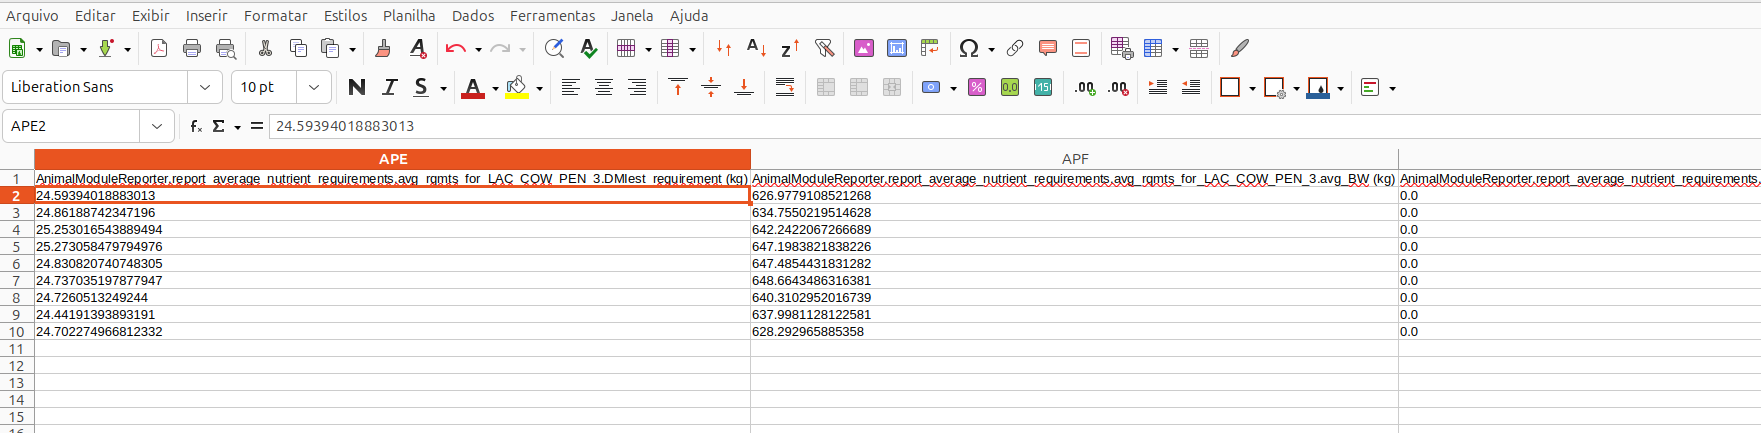
\includegraphics[width=\textwidth]{Images/exigencias_lac_cow_libreoffice.png}
    \caption{Colunas de exigências da baia de lactação no CSV de saída da simulação de 1 ano, abertas no LibreOffice Calc.}
    \label{fig:csv-exigencias}
\end{figure}

Em média, as vacas em lactação produziram 41,63 kg de leite e emitiram 373,8 g de metano por dia. A ração efetivamente aplicada pelo RuFaS teve, em média, 19,79 kg de silagem de milho, 6,43 kg do concentrado 303 e 0,25 kg de mineral, num total de 26,47 kg de MS por vaca, próxima da solução linear. Com os preços da \textbf{Tabela \ref{tab:precos}}, essa ração custa cerca de R\$ 24,75 por vaca por dia, ou R\$ 0,59 por kg de leite. Não houve redução de leite por dieta insuficiente em nenhuma formulação.

A \textbf{Tabela \ref{tab:comparacao}} compara a simulação com a dieta do programa linear e o caso base. Como os dois cenários usam a mesma semente e o mesmo período, a diferença entre eles se deve à dieta.

\begin{table}[htbp]
    \centering
    \caption{Caso base e dieta do programa linear em 1 ano (médias por vaca em lactação, por dia)}
    \label{tab:comparacao}
    \begin{tabular}{lrrr}
        \toprule
        & \textbf{Caso base} & \textbf{Dieta do PL} & \textbf{Diferença} \\
        \midrule
        \rowcolor{gray!15}
        Consumo de MS (kg) & 25,39 & 26,47 & +1,08 \\
        Leite (kg) & 41,29 & 41,63 & +0,34 \\
        \rowcolor{gray!15}
        Metano entérico (g) & 338,3 & 373,8 & +35,5 \\
        \bottomrule
    \end{tabular}
\end{table}

A dieta do programa linear manteve a produção de leite, que subiu 0,34 kg por vaca por dia, mas elevou a emissão de metano em 10,5\%, efeito da maior participação de silagem de milho e do maior consumo de matéria seca. O RuFaS marcou o cálcio como não atendido em 5 das 9 formulações, por diferenças inferiores a 0,0001 g: a restrição R6 está ativa na solução linear, e a exigência do grupo varia ligeiramente ao longo da simulação. Uma margem de segurança no modelo (por exemplo, cálcio $\geq$ 1,02 $\times$ exigência) evita esse efeito. Os testes de gordura e de ração válida falharam em todas as formulações nos dois cenários, e o de energia total passou apenas na primeira, também nos dois; portanto, essas falhas não decorrem da troca de dieta. O custo da ração original não pôde ser calculado com preços brasileiros, porque ela inclui alimentos que não constam da planilha (caroço de algodão e farelo de soja).

Como referência, o caso apresentado em aula \cite{slides:rufas}, uma execução do otimizador do RuFaS no padrão NASEM e em modo livre, para uma vaca de 740 kg com 150 dias de lactação e 35 kg de leite por dia, chegou a um custo mínimo de US\$ 4,65 por vaca por dia, ou US\$ 0,133 por kg de leite. Os valores não são diretamente comparáveis: aquele caso usa preços de mercado dos Estados Unidos em dólares e outro conjunto de ingredientes (silagens de milho e de leguminosa, feno de gramínea, milho moído, farelo de soja, caroço de algodão e mistura mineral), enquanto este trabalho usa preços brasileiros em reais.

% =====================================================================
\section{Avaliação do efeito econômico}\label{sec:economico}

O efeito econômico da dieta foi medido pela margem sobre o custo alimentar: a receita do leite menos o custo da alimentação, por vaca em lactação e por dia. Os valores foram calculados pelo \textit{script Scripts/\allowbreak avaliacao\_\allowbreak economica.py}, que lê os CSVs das simulações de 1 ano e usa a ração efetivamente aplicada pelo RuFaS (média das 9 formulações), os preços da \textbf{Tabela \ref{tab:precos}} e o preço do leite ao produtor em Goiás em agosto de 2026, de R\$ 2,9692 por litro \cite{website:cepealeite}. Com a densidade de 1,032 kg/L, esse preço equivale a R\$ 2,8771 por kg de leite, o mesmo valor adotado para o leite das bezerras.

Além do caso base e da dieta do programa linear, foi simulado um terceiro cenário, em que a ração das vacas em lactação é formulada pelo próprio otimizador do RuFaS em modo livre (\textbf{Seção \ref{sec:modolivre}}). O resultado está na \textbf{Tabela \ref{tab:economico}}.

\begin{table}[htbp]
    \centering
    \caption{Efeito econômico da dieta (médias por vaca em lactação, por dia, simulações de 1 ano)}
    \label{tab:economico}
    \begin{tabular}{lrrr}
        \toprule
        & \textbf{Caso base} & \textbf{Dieta do PL} & \textbf{Modo livre} \\
        \midrule
        \rowcolor{gray!15}
        Consumo de MS (kg) & 25,39 & 26,47 & 26,10 \\
        Leite (kg) & 41,29 & 41,63 & 41,38 \\
        \rowcolor{gray!15}
        Receita do leite (R\$) & 118,81 & 119,78 & 119,06 \\
        Custo da ração (R\$) & $\geq$ 33,38 & 24,75 & 24,47 \\
        \rowcolor{gray!15}
        Custo da ração por kg de leite (R\$) & $\geq$ 0,808 & 0,594 & 0,591 \\
        Margem sobre o custo alimentar (R\$) & $\leq$ 85,43 & 95,04 & 94,58 \\
        \bottomrule
    \end{tabular}
\end{table}

\newpage
No RuFaS, a dieta só altera a produção de leite quando não atende às exigências; nesse caso, o simulador reduz a produção. Isso não ocorreu em nenhuma formulação dos três cenários. A produção segue a curva de lactação de cada vaca, e as pequenas diferenças de leite entre os cenários acompanham a composição do rebanho: a média de dias em lactação foi de 152 dias no caso base, 148 na dieta do programa linear e 150 no modo livre. Por isso, a diferença econômica atribuível à dieta está no custo da ração.

A ração original contém caroço de algodão (58; 2,21 kg de MS por vaca) e farelo de soja (167; 3,97 kg de MS), que não constam da planilha de preços. Por isso, o custo do caso base na \textbf{Tabela \ref{tab:economico}} considera apenas os outros quatro alimentos (milho grão, silagem de milho, silagem de leguminosa e mistura mineral) e é um limite inferior do custo real. Mesmo assim, ele já supera em R\$ 8,63 o custo da dieta do programa linear. A dieta do programa linear reduz, portanto, o custo alimentar em pelo menos R\$ 8,63 por vaca por dia (26\%); com o rebanho médio de 89,8 vacas em lactação da simulação, a economia é de pelo menos R\$ 283 mil por ano. A margem sobre o custo alimentar da dieta do programa linear é de R\$ 95,04 por vaca por dia, cerca de R\$ 3,11 milhões por ano no rebanho.

O custo da ração aplicada (R\$ 24,75) é R\$ 0,44 maior que o da solução do programa linear (R\$ 24,31), porque o RuFaS reformula a ração a cada 45 dias com as exigências do momento, dentro da tolerância de 10\% em torno da dieta informada, e o consumo médio resultante (26,47 kg) é maior que o da solução (25,85 kg). A margem não inclui custos que não dependem da dieta, como mão de obra e energia, nem o aumento de 10,5\% na emissão de metano observado na \textbf{Seção \ref{sec:simulacao}}, que não tem preço no modelo.

\subsection{Comparação com o otimizador do RuFaS}\label{sec:modolivre}

Para comparar a dieta do programa linear com a do otimizador interno do RuFaS, foi simulado um cenário em modo livre, com os mesmos preços, período e semente das demais simulações. Os arquivos do cenário foram gerados pelo \textit{script Scripts/\allowbreak preparar\_\allowbreak cenarios.py}: o \textit{animal\_\allowbreak modo\_\allowbreak livre.json} define \textit{ration.user\_input} = \textit{false}, e o \textit{feed\_\allowbreak modo\_\allowbreak livre.json} lista na ração das vacas em lactação os nove alimentos candidatos do programa linear. Em modo livre, o RuFaS usa apenas a lista de alimentos de cada ração, sem os percentuais, e formula a ração de custo mínimo com o otimizador da \textbf{Seção \ref{sec:rufas}}. As rações de novilhas e de vacas pré-parto também passam a ser formuladas pelo otimizador, a partir dos alimentos já listados para elas. O cenário foi executado pelo comando da \textbf{Listagem \ref{lst:modolivre}} e terminou sem erros.

\begin{lstlisting}[caption={Execução do cenário em modo livre.}, label={lst:modolivre}]
python main.py -p GO_campo_dourado/_pipeline_task_manager_metadata_modo_livre.json -g
\end{lstlisting}

Entre os nove alimentos candidatos, o otimizador do RuFaS escolheu os mesmos três da solução do programa linear, em proporções quase iguais (\textbf{Tabela \ref{tab:modolivre}}).

\begin{table}[htbp]
    \centering
    \caption{Ração das vacas em lactação: programa linear e otimizador do RuFaS em modo livre}
    \label{tab:modolivre}
    \begin{tabular}{lrrrr}
        \toprule
        & \multicolumn{2}{c}{\textbf{Dieta do PL (aplicada)}} & \multicolumn{2}{c}{\textbf{Modo livre}} \\
        \textbf{Alimento} & \textbf{kg MS} & \textbf{\% da MS} & \textbf{kg MS} & \textbf{\% da MS} \\
        \midrule
        \rowcolor{gray!15}
        Silagem de milho (51) & 19,79 & 74,8 & 19,47 & 74,6 \\
        Mistura de subprodutos (303) & 6,43 & 24,3 & 6,37 & 24,4 \\
        \rowcolor{gray!15}
        Mistura mineral (301) & 0,25 & 1,0 & 0,25 & 1,0 \\
        \midrule
        \textbf{Total} & \textbf{26,47} & \textbf{100,0} & \textbf{26,10} & \textbf{100,0} \\
        \bottomrule
    \end{tabular}
\end{table}

O resultado confirma o modelo linear: o otimizador do RuFaS, que trata energia e proteína com as equações não lineares e resolve o problema por outro método, chegou à mesma dieta. O custo em modo livre foi R\$ 0,28 menor por vaca por dia, porque o otimizador ajusta a ração livremente às exigências de cada formulação, enquanto, com a dieta informada, ele fica limitado à tolerância de 10\% em torno dela, o que resultou em um consumo médio 0,37 kg maior. A diferença de margem entre os dois cenários (R\$ 0,45 a favor da dieta do programa linear) vem da produção de leite, que, como visto acima, reflete a composição do rebanho e não a dieta. Do ponto de vista econômico, as duas dietas são equivalentes.

% =====================================================================
\section{Análise de sensibilidade}\label{sec:sensibilidade}

A análise de sensibilidade verifica quanto a solução da \textbf{Seção \ref{sec:solucao}} depende dos dados de entrada, que são incertos: os preços variam com o mercado, e as exigências mudam ao longo da lactação. Ela foi feita pelo \textit{script Scripts/\allowbreak analise\_\allowbreak sensibilidade.py}, que usa o mesmo modelo PuLP do \textit{script} de geração do programa linear e o resolve novamente com o CBC em cada caso.

A solução ótima é definida por sua base: os alimentos que entram na dieta (51, 301 e 303) e as restrições ativas (R2, R4 e R6). Enquanto a base não muda, os preços-sombra e os custos reduzidos continuam válidos, e a composição da dieta muda de forma previsível. Para cada preço e cada exigência, o \textit{script} localiza por bisseção o valor em que a base muda, re-resolvendo o modelo a cada passo.

\subsection{Preços-sombra e custos reduzidos}

Os preços-sombra das restrições ativas e os custos reduzidos dos alimentos fora da dieta, obtidos do CBC, estão na \textbf{Tabela \ref{tab:duais}}. O preço-sombra indica quanto o custo diário aumenta se a exigência aumentar uma unidade; o custo reduzido indica quanto o preço de um alimento precisaria cair para ele entrar na dieta.

\begin{table}[htbp]
    \centering
    \caption{Preços-sombra e custos reduzidos (solução do CBC)}
    \label{tab:duais}
    \begin{tabular}{lr}
        \toprule
        \textbf{Item} & \textbf{Valor} \\
        \midrule
        \rowcolor{gray!15}
        Preço-sombra da energia líquida (R2) & 0,2646 R\$/Mcal \\
        Preço-sombra da proteína metabolizável (R4) & 0,0018 R\$/g \\
        \rowcolor{gray!15}
        Preço-sombra do cálcio (R6) & 0,0841 R\$/g \\
        \midrule
        Custo reduzido: silagem de capim-sudão (176) & 0,1357 R\$/kg MS \\
        \rowcolor{gray!15}
        Custo reduzido: milho grão (44) & 0,5046 R\$/kg MS \\
        Custo reduzido: feno de bermuda (18) & 1,0989 R\$/kg MS \\
        \rowcolor{gray!15}
        Custo reduzido: silagem de leguminosa (110) & 1,5340 R\$/kg MS \\
        Custo reduzido: feno misto (94) & 1,6840 R\$/kg MS \\
        \rowcolor{gray!15}
        Custo reduzido: silagem mista (100) & 1,8381 R\$/kg MS \\
        \bottomrule
    \end{tabular}
\end{table}

A silagem de capim-sudão é a alternativa mais próxima: basta seu preço cair cerca de 0,14 R\$/kg MS (de 0,7851 para 0,6494) para que ela passe a compor a dieta.

\subsection{Faixas de variação dos preços}

A \textbf{Tabela \ref{tab:faixascusto}} mostra os intervalos de preço em que a base ótima se mantém. Para os alimentos fora da dieta, o preço pode subir sem limite e só pode cair até o valor em que o custo reduzido se anula. Para os alimentos da dieta, as quantidades não mudam dentro da faixa, porque são definidas pelas três restrições ativas; muda apenas o custo total.

\begin{table}[htbp]
    \centering
    \caption{Faixas de preço com a mesma base ótima (R\$/kg MS)}
    \label{tab:faixascusto}
    \begin{tabular}{lrrrr}
        \toprule
        \textbf{Alimento} & \textbf{Atual} & \textbf{Mínimo} & \textbf{Máximo} & \textbf{Variação} \\
        \midrule
        \rowcolor{gray!15}
        Silagem de milho (51) & 0,6988 & 0,2499 & 0,8880 & $-$64,2\% a +27,1\% \\
        Mistura de subprodutos (303) & 1,2159 & 0,8230 & 2,9386 & $-$32,3\% a +141,7\% \\
        \rowcolor{gray!15}
        Mistura mineral (301) & 12,2904 & 0,0000 & 43,3760 & $-$100\% a +252,9\% \\
        \midrule
        Silagem de capim-sudão (176) & 0,7851 & 0,6494 & -- & $-$17,3\% a $+\infty$ \\
        \rowcolor{gray!15}
        Milho grão (44) & 1,2413 & 0,7367 & -- & $-$40,6\% a $+\infty$ \\
        Feno de bermuda (18) & 1,8207 & 0,7219 & -- & $-$60,4\% a $+\infty$ \\
        \rowcolor{gray!15}
        Silagem de leguminosa (110) & 2,5653 & 1,0313 & -- & $-$59,8\% a $+\infty$ \\
        Feno misto (94) & 2,5213 & 0,8373 & -- & $-$66,8\% a $+\infty$ \\
        \rowcolor{gray!15}
        Silagem mista (100) & 2,7486 & 0,9106 & -- & $-$66,9\% a $+\infty$ \\
        \bottomrule
    \end{tabular}
\end{table}

A dieta é robusta a variações de preço dos seus próprios ingredientes: a mistura de subprodutos pode mais que dobrar de preço, e a mistura mineral, mais que triplicar, sem mudar a composição. O ponto mais sensível é a relação entre as duas silagens. Uma alta de 27,1\% no preço da silagem de milho ou uma queda de 17,3\% no da silagem de capim-sudão já alteram a base, com a entrada da silagem de capim-sudão na dieta. Esse resultado deve ser lido com cautela, porque o preço da silagem de capim-sudão é um \textit{proxy}: o mesmo custo de produção por tonelada da silagem de milho (\textbf{Seção \ref{sec:ingredientes}}).

\subsection{Faixas de variação das exigências}

A \textbf{Tabela \ref{tab:faixasexig}} mostra as faixas das exigências em que a base se mantém e, portanto, em que os preços-sombra da \textbf{Tabela \ref{tab:duais}} são válidos. No caso do consumo de MS e da proteína metabolizável, a exigência foi variada em todas as restrições em que aparece (R1a e R1b; R3, R4 e R5). Para o cálcio, a base se mantém até pelo menos 10 vezes a exigência atual, limite da busca.

\begin{table}[htbp]
    \centering
    \caption{Faixas das exigências com a mesma base ótima}
    \label{tab:faixasexig}
    \begin{tabular}{lrrrr}
        \toprule
        \textbf{Exigência} & \textbf{Atual} & \textbf{Preço-sombra (R\$)} & \textbf{Faixa} & \textbf{Variação} \\
        \midrule
        \rowcolor{gray!15}
        Consumo de MS (kg) & 24,75 & 0 & 19,88 a 36,92 & $-$19,7\% a +49,2\% \\
        Energia líquida (Mcal) & 52,34 & 0,2646 por Mcal & 43,62 a 65,63 & $-$16,7\% a +25,4\% \\
        \rowcolor{gray!15}
        Proteína metabolizável (g) & 2.662,11 & 0,0018 por g & 2.504,99 a 4.841,55 & $-$5,9\% a +81,9\% \\
        Cálcio (g) & 67,00 & 0,0841 por g & $\geq$ 47,19 & $\geq$ $-$29,6\% \\
        \rowcolor{gray!15}
        Fósforo (g) & 63,41 & 0 & $\leq$ 65,91 & $\leq$ +3,9\% \\
        \bottomrule
    \end{tabular}
\end{table}

A energia é a exigência que mais pesa no custo: cada Mcal adicional custa R\$ 0,26 por vaca por dia, e o preço-sombra vale para variações de $-$16,7\% a +25,4\%, faixa que cobre as variações observadas entre as formulações da \textbf{Tabela \ref{tab:exigencias1ano}}. A proteína metabolizável tem preço-sombra baixo, mas a faixa é estreita para baixo: com uma exigência 5,9\% menor, a restrição R4 deixa de ser ativa. O fósforo não está ativo, mas a folga é pequena: um aumento de 3,9\% na exigência o tornaria ativo e mudaria a base ótima. Isso é relevante porque o RuFaS calcula duas exigências de fósforo e o modelo usa a maior delas (\textbf{Seção \ref{sec:modelo}}).

\subsection{Cenários de preços e de exigências}

A \textbf{Tabela \ref{tab:cenarios}} mostra o resultado do programa linear em cenários de preço e de exigência. As variações de $\pm$20\% nos preços são da ordem das oscilações de mercado de grãos e concentrados; as de $\pm$10\% nas exigências de energia, proteína, cálcio e fósforo representam vacas com produção maior ou menor que a média da baia. O último cenário aplica a margem de segurança de 2\% no cálcio sugerida na \textbf{Seção \ref{sec:simulacao}}.

\begin{table}[htbp]
    \centering
    \caption{Cenários de preços e de exigências (por vaca em lactação, por dia)}
    \label{tab:cenarios}
    \begin{tabular}{lrrL{5.6cm}}
        \toprule
        \textbf{Cenário} & \textbf{Custo (R\$)} & \textbf{Variação} & \textbf{Dieta (kg MS)} \\
        \midrule
        \rowcolor{gray!15}
        Solução de referência & 24,31 & -- & 51: 19,188 · 303: 6,404 · 301: 0,253 \\
        Silagem de milho (51) $-$20\% & 21,63 & $-$11,0\% & mesma \\
        \rowcolor{gray!15}
        Silagem de milho (51) +20\% & 26,99 & +11,0\% & mesma \\
        Subprodutos (303) $-$20\% & 22,75 & $-$6,4\% & mesma \\
        \rowcolor{gray!15}
        Subprodutos (303) +20\% & 25,87 & +6,4\% & mesma \\
        Mineral (301) +20\% & 24,93 & +2,6\% & mesma \\
        \rowcolor{gray!15}
        Milho grão (44) $-$20\% & 24,31 & 0,0\% & mesma \\
        Silagem de capim-sudão (176) $-$20\% & 24,13 & $-$0,7\% & 51: 13,084 · 176: 8,514 · 303: 5,733 · 301: 0,217 \\
        \rowcolor{gray!15}
        Exigências $-$10\% & 21,88 & $-$10,0\% & 51: 17,269 · 303: 5,763 · 301: 0,228 \\
        Exigências +10\% & 26,74 & +10,0\% & 51: 21,106 · 303: 7,044 · 301: 0,279 \\
        \rowcolor{gray!15}
        Cálcio $\times$ 1,02 & 24,42 & +0,5\% & 51: 19,189 · 303: 6,403 · 301: 0,263 \\
        \bottomrule
    \end{tabular}
\end{table}

O custo da dieta responde quase linearmente às exigências: variações de 10\% nas exigências de nutrientes mudam o custo em 10\%, sem mudar os ingredientes. A silagem de milho é o insumo de maior impacto, pois responde por mais da metade do custo: uma variação de 20\% no seu preço muda o custo diário em 11\%. Uma queda de 20\% no preço do milho grão não o traz para a dieta, porque seria preciso uma queda de 40,6\%. Já uma queda de 20\% no preço da silagem de capim-sudão muda a dieta, com a substituição de parte da silagem de milho, mas reduz o custo em apenas 0,7\%. Esse cenário foi simulado no RuFaS na \textbf{Seção \ref{sec:sudao}}. A margem de segurança no cálcio custa R\$ 0,11 por vaca por dia (0,5\%) e evita que o RuFaS marque o cálcio como não atendido por diferenças mínimas.

\subsection{Simulação de um cenário no RuFaS}\label{sec:sudao}

Os cenários anteriores avaliam apenas o programa linear. Para medir o efeito de uma mudança de base no rebanho simulado, o cenário em que a silagem de capim-sudão fica 20\% mais barata (R\$ 0,6281 por kg de MS) foi simulado no RuFaS. Os arquivos foram gerados pelo \textit{script Scripts/\allowbreak preparar\_\allowbreak cenarios.py}, que resolve o programa linear com o novo preço e grava a dieta resultante (silagem de milho 47,5\%, silagem de capim-sudão 30,9\%, mistura de subprodutos 20,8\% e mistura mineral 0,8\% da MS) e o novo preço no \textit{feed\_\allowbreak sens\_\allowbreak sudao.json}. A simulação usou o mesmo período e a mesma semente das demais e terminou sem erros. A \textbf{Tabela \ref{tab:sudao}} compara o resultado com o da simulação com a dieta do programa linear original, que não usa silagem de capim-sudão e, portanto, tem o mesmo custo com o novo preço.

\begin{table}[htbp]
    \centering
    \caption{Efeito da queda de 20\% no preço da silagem de capim-sudão no RuFaS (médias por vaca em lactação, por dia)}
    \label{tab:sudao}
    \begin{tabular}{lrrr}
        \toprule
        & \textbf{Dieta do PL} & \textbf{Dieta com capim-sudão} & \textbf{Diferença} \\
        \midrule
        \rowcolor{gray!15}
        Custo no programa linear (R\$) & 24,31 & 24,13 & $-$0,18 \\
        Consumo de MS aplicado (kg) & 26,47 & 27,74 & +1,27 \\
        \rowcolor{gray!15}
        Custo da ração aplicada (R\$) & 24,75 & 24,15 & $-$0,60 \\
        Leite (kg) & 41,63 & 41,03 & $-$0,60 \\
        \rowcolor{gray!15}
        Metano entérico (g) & 373,8 & 453,6 & +79,8 \\
        Margem sobre o custo alimentar (R\$) & 95,04 & 93,89 & $-$1,15 \\
        \bottomrule
    \end{tabular}
\end{table}

A troca de base reduziu o custo da ração aplicada em R\$ 0,60 por vaca por dia, mais do que o previsto pelo programa linear (R\$ 0,18), porque o RuFaS reformula a ração a cada formulação. Não houve redução de leite por dieta insuficiente: a queda de 0,60 kg de leite acompanha a composição do rebanho, com média de 156 dias em lactação, contra 148 na simulação com a dieta do programa linear, e não deve ser atribuída à dieta (\textbf{Seção \ref{sec:economico}}). O efeito mais claro da troca é ambiental: a silagem de capim-sudão tem mais fibra (66,6\% de FDN, contra 40,9\% da silagem de milho), o consumo de MS aumentou 1,27 kg e a emissão de metano entérico subiu 21,3\%. A economia de R\$ 0,60 por vaca por dia, cerca de 2,4\% do custo da ração, vem acompanhada de um aumento expressivo de emissões, que a função objetivo de custo mínimo não considera.

% =====================================================================
\newpage
\section{Limitações e conclusões}\label{sec:conclusao}

O trabalho mostrou que é possível reescrever o problema de formulação de ração do RuFaS como um programa linear, com baixo erro de linearização. A simulação, executada como um exemplo prático, deu ao grupo uma noção de como um problema real pode ser resolvido por meio de técnicas de programação linear.

Durante o desenvolvimento do projeto, o grupo enfrentou dificuldades técnicas para instalar e executar o RuFaS, devido às constantes atualizações do repositório, que geraram instabilidades nas versões recentes. As simulações só puderam ser feitas a partir da segunda metade do cronograma, após a recuperação de uma versão anterior e estável do código. Por isso, não há certeza de que o exercício tenha sido concluído exatamente como solicitado, e o grupo permanece aberto a correções.

\newpage
%\bibliographystyle{plain}	%inclui as referẽncias em ordem alfabética do sobrenome do autor
%\bibliographystyle{unsrt}	%inclui as referẽncias em ordem de aparição das citações
\bibliographystyle{ieeetr}	%inclui as referẽncias no padrão IEEE (em ordem de aparição)
\bibliography{references}

\newpage
\appendix
\renewcommand{\thesection}{Apêndice \Alph{section}}

\section{Arquivos do trabalho}\label{sec:anexoarquivos}

O trabalho foi desenvolvido em Python sobre o simulador RuFaS. A \textbf{Tabela \ref{tab:arquivos}} lista os arquivos produzidos ou alterados.

\begin{table}[htbp]
    \centering
    \caption{Arquivos do trabalho}
    \label{tab:arquivos}
    \begin{tabular}{L{7.2cm}L{9.2cm}}
        \toprule
        \textbf{Arquivo} & \textbf{Função} \\
        \midrule
        \rowcolor{gray!15}
        \textit{Scripts/\allowbreak ingredientes\_\allowbreak racoes\_\allowbreak GO\_\allowbreak campo\_\allowbreak dourado.xlsx} & Ingredientes, composição, preços, fontes e conversões \\
        \textit{sincronizar\_\allowbreak planilha\_\allowbreak rufas.py} & Transfere preços e composição da planilha para o \textit{feed.json} e o \textit{NASEM\_Comp.csv} \\
        \rowcolor{gray!15}
        \textit{Scripts/\allowbreak gerar\_\allowbreak modelo\_\allowbreak pl.py} & Monta o programa linear com o PuLP, resolve com o CBC e mede o erro de linearização \\
        \textit{Scripts/modelo\_pl\_lac\_cow.md} & Formulação do modelo para leitura \\
        \rowcolor{gray!15}
        \textit{Scripts/modelo\_pl\_lac\_cow.lp} & Modelo no formato CPLEX LP, para \textit{solvers} \\
        \textit{Scripts/\allowbreak analise\_\allowbreak sensibilidade.py} & Calcula preços-sombra, faixas de custo e de exigências e os cenários da análise de sensibilidade \\
        \rowcolor{gray!15}
        \textit{Scripts/\allowbreak avaliacao\_\allowbreak economica.py} & Calcula custo da ração, receita do leite e margem sobre o custo alimentar das simulações \\
        \textit{Scripts/\allowbreak preparar\_\allowbreak cenarios.py} & Gera os arquivos de entrada dos cenários em modo livre e de sensibilidade \\
        \rowcolor{gray!15}
        \textit{build\_pdf\_report.py} & Gera o relatório em PDF dos ingredientes a partir da planilha \\
        \textit{GO\_campo\_dourado/} & Arquivos de entrada da fazenda, com as correções da \textbf{Seção \ref{sec:preparacao}} \\
        \rowcolor{gray!15}
        \textit{GO\_\allowbreak campo\_\allowbreak dourado/\allowbreak *\_caso\_base.json} & Arquivos do cenário do caso base, com a ração original (\textbf{Seção \ref{sec:exigencias}}) \\
        \textit{GO\_\allowbreak campo\_\allowbreak dourado/\allowbreak *\_modo\_livre.json} & Arquivos do cenário em modo livre do otimizador do RuFaS (\textbf{Seção \ref{sec:modolivre}}) \\
        \rowcolor{gray!15}
        \textit{GO\_\allowbreak campo\_\allowbreak dourado/\allowbreak *\_sens\_sudao.json} & Arquivos do cenário de sensibilidade com a silagem de capim-sudão (\textbf{Seção \ref{sec:sensibilidade}}) \\
        \textit{output/\allowbreak output\_\allowbreak filters/\allowbreak csv\_\allowbreak dieta\_\allowbreak otimizacao.txt} & Filtro de saída com as variáveis de dieta, exigências, leite, metano e esterco \\
        \bottomrule
    \end{tabular}
\end{table}

% TODO: incluir o link do repositório do trabalho.

\newpage
\section{Matriz de coeficientes do programa linear}\label{sec:anexomatriz}

\begin{table}[htbp]
    \centering
    \caption{Matriz de coeficientes (por kg de MS de cada alimento)}
    \label{tab:matriz}
    \resizebox{\textwidth}{!}{%
    \begin{tabular}{lrrrrrrrrrcr}
        \toprule
        & $x_{18}$ & $x_{44}$ & $x_{51}$ & $x_{94}$ & $x_{100}$ & $x_{110}$ & $x_{176}$ & $x_{301}$ & $x_{303}$ & & \textbf{L. dir.} \\
        \midrule
        \rowcolor{gray!15}
        Custo $Z$ & 1,8207 & 1,2413 & 0,6988 & 2,5213 & 2,7486 & 2,5653 & 0,7851 & 12,2904 & 1,2159 & min & -- \\
        R1a & 1 & 1 & 1 & 1 & 1 & 1 & 1 & 1 & 1 & $\geq$ & 17,3267 \\
        \rowcolor{gray!15}
        R1b & 1 & 1 & 1 & 1 & 1 & 1 & 1 & 1 & 1 & $\leq$ & 32,1782 \\
        R2 & 1,7953 & 2,3165 & 2,0709 & 1,9188 & 1,8844 & 1,8534 & 1,6394 & $-$0,1875 & 1,9763 & $\geq$ & 52,3437 \\
        \rowcolor{gray!15}
        R3 & 63,8324 & 99,1059 & 71,1721 & 71,7214 & 70,6693 & 81,4868 & 70,9403 & 4,7200 & 326,3928 & $\geq$ & 2.662,11 \\
        R4 & 67,8272 & 58,5307 & 50,2368 & 94,8550 & 106,1834 & 123,9203 & 56,9029 & 4,7200 & 265,0060 & $\geq$ & 2.662,11 \\
        \rowcolor{gray!15}
        R5 & 63,8324 & 99,1059 & 71,1721 & 71,7214 & 70,6693 & 81,4868 & 70,9403 & 4,7200 & 326,3928 & $\leq$ & 3.993,17 \\
        R6 & 1,4730 & 0,2100 & 0,7110 & 1,8750 & 2,6100 & 3,7620 & 1,3380 & 146,5850 & 2,5320 & $\geq$ & 66,998 \\
        \rowcolor{gray!15}
        R7 & 1,2480 & 2,1630 & 1,4848 & 2,1056 & 2,1824 & 2,2464 & 1,7024 & 18,5600 & 5,1100 & $\geq$ & 63,410 \\
        R8 & 40,41 & $-$15,24 & 15,93 & 29,69 & 26,23 & 18,20 & 41,62 & $-$24,86 & $-$1,12 & $\geq$ & 0 \\
        \rowcolor{gray!15}
        R9 & 20,41 & $-$35,24 & $-$4,07 & 9,69 & 6,23 & $-$1,80 & 21,62 & $-$44,86 & $-$21,12 & $\leq$ & 0 \\
        R10 & 50,41 & $-$15,00 & 25,93 & 39,69 & 36,23 & 28,20 & 51,62 & $-$15,00 & $-$15,00 & $\geq$ & 0 \\
        \rowcolor{gray!15}
        R11 & $-$5,0720 & $-$3,1550 & $-$4,0840 & $-$3,6060 & $-$2,9620 & $-$4,1280 & $-$4,3080 & $-$6,9988 & $-$1,7791 & $\leq$ & 0 \\
        \bottomrule
    \end{tabular}}
\end{table}

\end{document}
